\documentclass{standalone}
\usepackage[dvipsnames,svgnames,x11names]{xcolor}
\usepackage{tikz}
\usepackage{pgfplots}
\pgfplotsset{compat = 1.12}
\usepackage{../thesismath}
\begin{document}
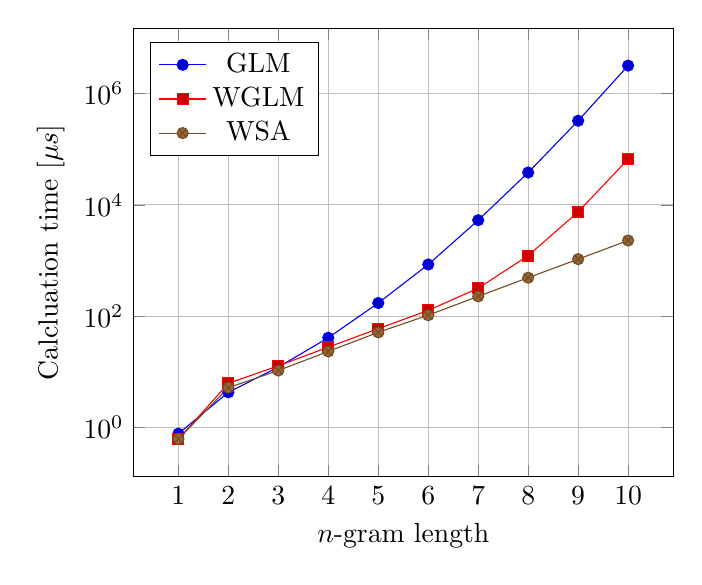
\begin{tikzpicture}[baseline]

\begin{axis}[
  xlabel = {$n$-gram length},
  xtick = {1, ..., 10},
  ylabel = {Calcluation time [${\mu}s$]},
  ymode = log,
  %yticklabel pos = right,
  minor y tick num = 4,
  grid = major,
  legend entries = {{GLM}, {WGLM}, {WSA}},
  legend pos = north west,
]

% GLM
\addplot table {
  n   us
  % sampled at N = 1000
  1   0.776
  2   4.296
  3   12.188
  4   40.981
  5   172.271
  % sampled at N = 100
  6   848.550
  7   5297.308
  % sampled at N = 10
  8   38045.228
  9   323947.490
  % sampled at N = 1
  10  3168612.887
};

% WGLM
\addplot table {
  n   us
  % sampled at N = 1000
  1   0.618
  2   6.223
  3   12.855
  4   27.786
  5   59.746
  % sampled at N = 100
  6   126.934
  7   317.936
  8   1223.680
  9   7463.531
  10  66226.605
};

% WSA
\addplot table {
  n   us
  % sampled at N = 1000
  1   0.624
  2   5.200
  3   10.572
  4   23.295
  5   51.307
  % sampled at N = 100
  6   104.217
  7   226.905
  8   491.327
  9   1056.845
  10  2287.351
};

\end{axis}

\end{tikzpicture}
\end{document}
